% =====================================================================
%  Rosetta — arXiv preprint
%  Build:  pdflatex rosetta && bibtex rosetta && pdflatex rosetta && pdflatex rosetta
%
%  Status: sections 1-9 and 12 are drafted from the implementation.
%  Section 10 reports E1-E5, all measured.
%  Section 11 (case study) is written from E6; 13 (related work) and 14 remain.
%  Every \todo{} marks something that does not exist in the repo yet;
%  `make todo` lists them. See OUTLINE.md for the plan.
% =====================================================================
\documentclass[11pt,a4paper]{article}

\usepackage[utf8]{inputenc}
\usepackage[T1]{fontenc}
\usepackage[english]{babel}
\usepackage{lmodern}
\usepackage{microtype}
\usepackage[margin=2.6cm]{geometry}
\usepackage{amsmath,amssymb}
\usepackage{booktabs}
\usepackage{longtable}
\usepackage{graphicx}
\usepackage{listings}
\usepackage{xcolor}
\usepackage{tikz}
\usetikzlibrary{arrows.meta,positioning,fit,backgrounds}
\usepackage[hidelinks]{hyperref}

% --- drafting aids -------------------------------------------------
\newcommand{\todo}[1]{\textcolor{red}{\textbf{[TODO: #1]}}}
\newcommand{\gap}[1]{\textcolor{orange}{\textsf{\small$\langle$#1$\rangle$}}}

% --- code listings -------------------------------------------------
\definecolor{codebg}{gray}{0.96}
\lstdefinestyle{cpp}{
  language=C++, basicstyle=\ttfamily\footnotesize,
  keywordstyle=\color{blue!60!black}, commentstyle=\color{gray},
  stringstyle=\color{green!40!black},
  backgroundcolor=\color{codebg}, frame=none,
  showstringspaces=false, breaklines=true, columns=fullflexible,
  morekeywords={consteval,constexpr,requires,concept,template,auto,co_await}
}
\lstset{style=cpp}

% --- shorthands ----------------------------------------------------
\newcommand{\rosetta}{\textsc{Rosetta}}
\newcommand{\code}[1]{\texttt{\small #1}}

% =====================================================================
\title{\textbf{Reflection as an Interface Description Language:\\
Static and Dynamic Multi-Language Projections of C++ APIs}}

\author{
  Frantz Maerten\\
  Look Up Geoscience\\
  \small\texttt{fmaerten@gmail.com}
  % \and
  % Bruno L\'evy\\
  % Inria Nancy\\
  % \small\texttt{Bruno.Levy@inria.fr}
}

\date{\today}

\begin{document}
\maketitle

% =====================================================================
\begin{abstract}
Exposing a C++ library to another language is normally paid for once per target:
a hand-written \code{pybind11} module for Python, an N-API layer for Node, a
\code{sol2} usertype for Lua, a marshalling shim for C\#, and a moc-annotated
class hierarchy for a Qt user interface. Each of these restates, in a different
notation, information the C++ compiler already has.

We present \rosetta, a system that reads that information once --- through
C++26 static reflection (P2996) over \emph{unmodified} headers --- into a
target-neutral intermediate representation (IR), and then \emph{projects} that
representation two ways. The \emph{static} projection emits ordinary C++ source
for nineteen targets; for seventeen of them the emitted code contains no
reflection at all and builds with any released C++20 compiler, rather than the
experimental fork reflection itself requires. The \emph{dynamic} projection emits the same information as
static metadata tables, giving a runtime meta-object model that scripts and user
interfaces query by name, without having been compiled against the library's
headers.

The central observation is that these are not two features but one mechanism
seen from two sides, differing only in \emph{when} names are resolved. We
demonstrate this with a measurable consequence: five targets whose binding
surfaces are name-keyed --- Lua, Node, WebAssembly, C\# and Java --- must discard
C++ overload sets at generation time, yet recover them in full through the
dynamic projection, because resolution moves from generation time to call time.
The expressiveness difference between targets is therefore not a property of the
target language but of its resolution time.

\rosetta{} additionally treats binding coverage as a first-class artifact: every
member that is not exposed is recorded, with a machine-readable reason, in a
\code{coverage.json} that can be diffed across revisions. On a controlled
288-method API, the five name-keyed targets bind 96 methods however many
overloads are declared, while the late-bound projection reaches all 288 ---
two thirds of the interface recovered by deferring resolution alone. Pointed at
an unmodified third-party mesh library and asked to bind its entire public
namespace unattended, the pipeline reaches 75\% of what it is given, and the
reason the rest fails is concentrated rather than diffuse: a quarter of that
library's declared surface is templates, and 85\% of those sit in its vector and
matrix value types rather than in the algorithms a caller invokes.
\end{abstract}

\noindent\textbf{Keywords:} static reflection, C++26, language bindings,
intermediate representation, meta-object protocol, scientific software.

% =====================================================================
\section{Introduction}
\label{sec:intro}

A scientific C++ library rarely stays in C++. Its users want it from Python for
analysis, from Julia for numerics, from a notebook, from a browser, from behind
a REST endpoint, and from a graphical interface that lets them move a slider and
see a result. Each of these is, today, a separate engineering project with its
own idioms, its own failure modes and its own maintenance burden --- and each
one begins by restating facts that the C++ compiler already knows perfectly
well: that \code{Mesh} has a field named \code{opacity} of type \code{double},
that \code{at} is overloaded on \code{int} and on \code{int,int}, that
\code{Solver} derives from \code{Operator}.

That restatement is the cost this paper is about. It is paid $N$ times for $N$
targets, it drifts silently when the C++ API changes, and it is the reason many
scientific libraries have exactly one binding --- usually Python --- and no
plausible route to a second.

C++26 static reflection~\cite{p2996} changes what is possible here, because for
the first time the information is available \emph{from inside the language},
with the compiler's own answers to the questions that a third-party parser has
to re-derive: which overload is hidden by a derived declaration, which special
members are implicitly declared, which base is public, what a template
specialisation is actually spelled. A system built on it does not need to carry
a C++ front-end of its own.

But reflection alone does not produce bindings, and treating it as a
better-parser is to under-use it. This paper argues a stronger position:

\begin{quote}\itshape
Static reflection can serve as a language-independent interface description
mechanism. One reflective pass over an unmodified C++ library yields an
intermediate representation from which \emph{both} reflection-free static
bindings \emph{and} a persistent runtime meta-object model can be projected ---
and the two projections differ only in when name resolution happens.
\end{quote}

\paragraph{Contributions.}
\begin{enumerate}
  \item \textbf{A reflection-derived, target-neutral IR.} A single
    \code{consteval} walk over a type hands each member, together with its full
    annotation pack, to a visitor. Backends never see \code{std::meta::info}
    (Section~\ref{sec:ir}).
  \item \textbf{A static projection to nineteen heterogeneous targets} ---
    language bindings, documentation, schemas and user interfaces --- from that
    one description (Section~\ref{sec:static}).
  \item \textbf{Reflection-free deployment.} Reflection is confined to the
    generation stage: for seventeen of the nineteen targets the emitted code
    requires only C++20, so it builds with any released compiler rather than
    the experimental fork reflection itself needs
    (Section~\ref{sec:pipeline}). The two exceptions are deliberate and are
    stated in Section~\ref{sec:limitations}.
  \item \textbf{A dynamic projection}: the same IR written out as static
    metadata tables, yielding a runtime meta-object model that a script or a
    GUI queries by name without knowing the C++ types (Section~\ref{sec:dynamic}).
  \item \textbf{Resolution time as the organising axis.} We show that
    expressiveness lost by early-binding targets is recovered by the late-bound
    projection, and quantify it (Section~\ref{sec:resolution}).
  \item \textbf{Coverage as a first-class, machine-readable artifact}: what was
    not bound, and why (Section~\ref{sec:coverage}).
\end{enumerate}

\paragraph{What we do not claim.}
We do not claim that \rosetta{} produces better Python bindings than a
hand-written \code{pybind11} module; an expert with unlimited time will always
win on one target. We claim that the \emph{per-target} cost is what \rosetta{}
removes. Nor do we claim the meta-object model itself is novel --- Qt's
meta-object system~\cite{qt}, Graphite's GOM~\cite{graphite}, Unreal's UObject
reflection~\cite{unreal} and Objective-C all long predate it. The novelty is
that the model is \emph{derived automatically, by the compiler, from unmodified
headers}, and that it shares its description with the static bindings.

% =====================================================================
\section{Motivation: the per-target cost}
\label{sec:motivation}

\subsection{One method, five notations}

Consider a single member function of a small numerical class --- a flat buffer
of scalars grouped into items:

\begin{lstlisting}[caption={The declaration. Everything below is derived from it.},label={lst:decl}]
namespace serie {
    class Serie {
    public:
        std::size_t itemSize() const;   // scalars per item
        // ...
    };
}
\end{lstlisting}

Listing~\ref{lst:five} is what exposing that one function costs in five host
environments. Each line is taken verbatim from \rosetta's own output, but
nothing about them is \rosetta-specific --- they are what a developer writes by
hand, and what the corresponding hand-written module contains.

\begin{lstlisting}[caption={The same member function, five times.},label={lst:five}]
// pybind11
c.def("itemSize", &serie::Serie::itemSize, "Scalars per item: ...");

// N-API (Node)
props.push_back(This::InstanceMethod<&This::call_method<
                    &serie::Serie::itemSize>>("itemSize"));

// embind (WebAssembly)
.function("itemSize", static_cast<unsigned long (serie::Serie::*)() const>(
                          &serie::Serie::itemSize))

// jlcxx (Julia)
c.method("itemSize", static_cast<unsigned long (serie::Serie::*)() const>(
                         &serie::Serie::itemSize));

// sol2 (Lua)
c["itemSize"] = &serie::Serie::itemSize;
\end{lstlisting}

Five notations, and every one of them encodes the same three facts: \emph{which
C++ entity} is being exposed, \emph{what name} it takes in the host language,
and --- explicitly in the embind and jlcxx cases, implicitly in the others ---
\emph{what its signature is}. All three are already known to the compiler that
just parsed Listing~\ref{lst:decl}. None of them is a design decision; they are
transcription.

The two lines carrying an explicit \code{static\_cast} are worth noticing,
because they show the transcription failing in a way that is easy to get wrong:
\code{\&Serie::itemSize} names an \emph{overload set}, not a function, so a
target that cannot take an overload set has to spell out the signature to pick a
member. That spelling must then track the declaration by hand. It is exactly the
kind of duplicated fact that drifts.

\subsection{The cost is differential, not just initial}

Writing five bindings once is a bounded, if tedious, expense. The recurring one
is that the C++ API moves. A method added to \code{Serie} must be added five
more times, in five notations, in five files; a renamed parameter, a changed
return type or a new overload propagates the same way.

We measure this in Section~\ref{sec:e2}: across three targets, hand-writable binding
code grows at 67 lines per class, and four generated source files change on
\emph{every} version bump of the library. Nothing about the arithmetic depends
on the bindings being generated --- 67 lines per class is what a developer would
otherwise be maintaining.

Worse, the failure mode is silent. A method that nobody remembered to add to the
Lua module is indistinguishable, from outside, from a method that was never
supposed to be there: the module simply does not have it, and no build step
objects. This is the observation that motivates making binding coverage an
explicit, machine-readable artifact rather than an inference from what happens
to compile (Section~\ref{sec:coverage}).

\subsection{The second-order problem: interfaces over the same facts}

A binding is not the only consumer of a type's structure. A property panel needs
to know that \code{Serie} has an \code{itemSize}, what type it is, whether it is
writable, and what range it may take. A console inspector, a QML view, an
immediate-mode debug overlay and a REST schema all need the same. Each is a
further restatement of the same facts, and because each targets a different
toolkit, each is written separately.

This is not hypothetical: it is what \rosetta's own repository looked like.
Before the dynamic projection existed, five hand-written C++ walkers traversed
the same metadata, one per consumer --- a console interpreter (446 lines), a Qt
property panel (401), a Qt main window (235), an ImGui runtime (331) and a QML
reflected object (102): about 1\,500 lines expressing one idea five times, each
of which had to be revisited whenever the metadata changed shape.

The measure of how much of that was accidental rather than essential: the Qt
property panel's 401 lines of C++ become 30 lines of Python once the metadata is
reachable from the host language (Section~\ref{sec:dynamic}). What the C++ walkers were
mostly doing was not building widgets --- it was re-deriving structure that
something else already knew.

\subsection{The requirement}

Both problems have the same shape. The information is available exactly once,
in the compiler, at the moment it parses the header; and it is then re-entered
by hand, once per consumer, in a notation that consumer happens to use. So:

\begin{quote}\itshape
The description should be extracted once, by the entity that already has it, in
a form no consumer's notation is privileged over --- and then projected, as many
times as there are consumers.
\end{quote}

Static reflection makes the extraction possible. The rest of this paper is about
what the intermediate form has to record for the projections to be faithful, and
what happens when the consumers disagree about what they can express.

% =====================================================================
\section{Background: C++26 static reflection, and what it forces}
\label{sec:background}

P2996~\cite{p2996} introduces \code{std::meta::info}, a reflection value
denoting a program entity, together with \code{consteval} queries over it
(\code{members\_of}, \code{type\_of}, \code{identifier\_of}, \dots) and
\emph{splicing}, which turns a reflection value back into a usable declaration.

Two properties matter for what follows.

\paragraph{The compiler's answers, not a parser's.}
Because the queries run inside a real compilation of the user's headers, they
report what the language actually decided. Listing~\ref{lst:hiding} is the canonical
case: \code{Derived::f(double)} hides both base overloads, and a C++ caller
without a \code{using Base::f;} cannot reach them. \rosetta{} binds exactly
\code{f(double)}, and records the two hidden declarations as drops. A system
built on an independent C++ parser must re-implement name hiding, access
control, implicit special-member declaration and template instantiation, and
will diverge from the compiler in the corners.

\begin{lstlisting}[caption={Name hiding is a compiler decision, not a syntactic one.},label={lst:hiding}]
struct Base    { int f(int) const; int f(int, int) const; };
struct Derived : Base { int f(double) const; };
// Derived binds only f(double); the two Base overloads are recorded
// as `hidden_by_derived` drops.
\end{lstlisting}

\paragraph{The constraint that shapes everything else.}
Reflection answers questions \emph{at the compile time of a program that
includes the user's headers}. It cannot be queried from a script, a build system
or a configuration file. Therefore, to learn the shape of a type, something must
\emph{compile}; and to write the answers to disk, that something must
\emph{run}. Compile-then-run is not an implementation choice --- it is the only
shape this can have, and it is why \rosetta{} is a pipeline rather than a
command. Section~\ref{sec:pipeline} makes that pipeline explicit.

\paragraph{Availability.} P2996 is implemented in \code{clang-p2996}, a research
fork. Section~\ref{sec:limitations} states precisely where this dependency bites and
where it does not.

% =====================================================================
\section{Architecture: a two-stage pipeline}
\label{sec:pipeline}

\begin{figure}[t]
\centering
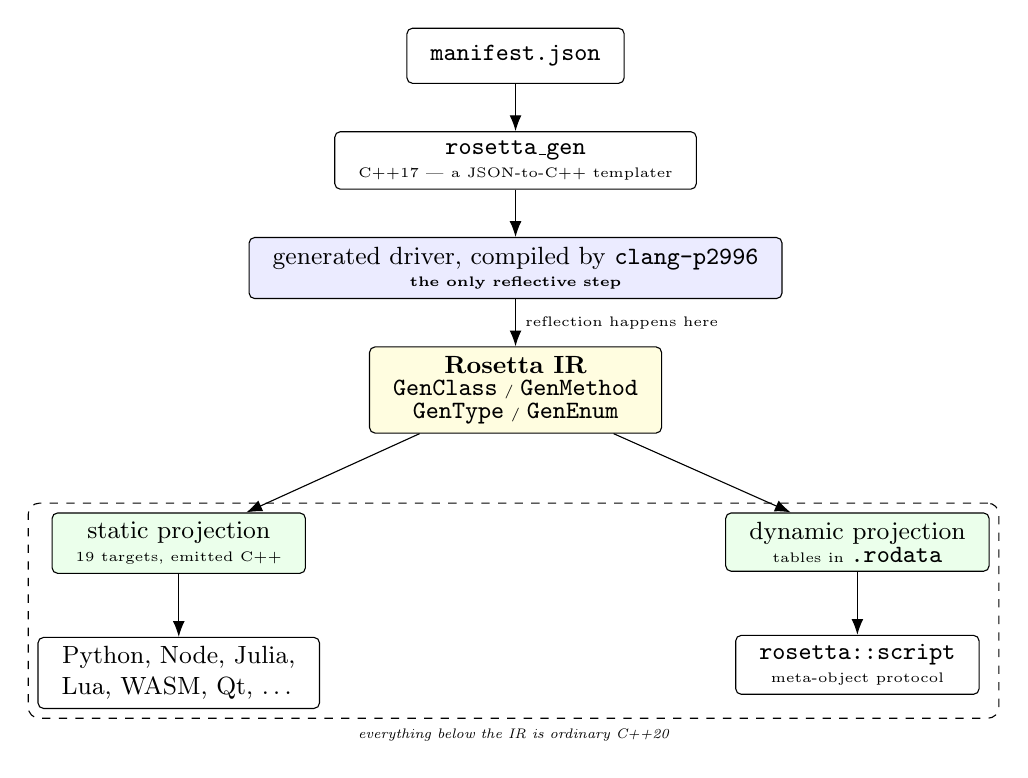
\begin{tikzpicture}[
  node distance=6mm,
  box/.style={draw, rounded corners=2pt, align=center, font=\small,
              minimum height=7mm, inner xsep=3mm},
  refl/.style={box, fill=blue!8},
  noreflect/.style={box, fill=green!8},
  arr/.style={-{Latex[length=2mm]}}
]
\node[box] (man) {\code{manifest.json}};
\node[box, below=of man] (gen) {\code{rosetta\_gen}\\[-1mm]{\tiny C++17 --- a JSON-to-C++ templater}};
\node[refl, below=of gen] (drv) {generated driver, compiled by \code{clang-p2996}\\[-1mm]{\tiny \textbf{the only reflective step}}};
\node[box, below=of drv, fill=yellow!12] (ir) {\textbf{Rosetta IR}\\[-1mm]{\tiny \code{GenClass} / \code{GenMethod}}\\[-1mm]{\tiny \code{GenType} / \code{GenEnum}}};

\node[noreflect, below left=10mm and 8mm of ir] (stat) {static projection\\[-1mm]{\tiny 19 targets, emitted C++}};
\node[noreflect, below right=10mm and 8mm of ir] (dyn) {dynamic projection\\[-1mm]{\tiny tables in \code{.rodata}}};

\node[box, below=8mm of stat] (langs) {Python, Node, Julia,\\ Lua, WASM, Qt, \dots};
\node[box, below=8mm of dyn] (mop) {\code{rosetta::script}\\[-1mm]{\tiny meta-object protocol}};

\draw[arr] (man) -- (gen);
\draw[arr] (gen) -- (drv);
\draw[arr] (drv) -- node[right,font=\tiny] {reflection happens here} (ir);
\draw[arr] (ir) -- (stat);
\draw[arr] (ir) -- (dyn);
\draw[arr] (stat) -- (langs);
\draw[arr] (dyn) -- (mop);

\begin{scope}[on background layer]
  \node[draw, dashed, rounded corners, fit=(stat)(dyn)(langs)(mop),
        label={[font=\tiny\itshape]below:everything below the IR is ordinary C++20}] {};
\end{scope}
\end{tikzpicture}
\caption{The pipeline. Reflection occurs in exactly one place. The IR is the
pivot: to its left the static projection, to its right the dynamic one. Nothing
reflection-flavoured survives into the emitted artifacts.}
\label{fig:pipeline}
\end{figure}

\paragraph{Stage 0 --- the templater.}
\code{rosetta\_gen} reads a \code{manifest.json} and emits a C++ driver program,
a header that includes the user's types, and a \code{CMakeLists.txt}. It
performs no reflection and builds with any C++17 compiler; it never opens
the user's headers, only copies their names into the driver it writes. Its
purpose is that what a project author writes is a \emph{manifest}, not a
program.

\paragraph{Stage 1 --- reflect and emit.}
The driver is compiled with \code{clang-p2996} and executed. During its
compilation the reflective walk runs; during its execution it writes files.
This is the compile-then-run sequence Section~\ref{sec:background} showed to be
unavoidable.

\paragraph{Stages 2--3 --- build and load.}
The emitted projects are ordinary C++20. They are configured and built with a
released compiler and loaded by their host runtimes. Each stage therefore has a
different and decreasing language requirement: C++17 to build the templater,
C++26 to run the reflective driver, C++20 to build what it produced.

\paragraph{The library is read twice.}
Table~\ref{tab:twice} states the property that makes reflection-free deployment
possible: the first pass \emph{describes} the types and needs C++26; the second
\emph{calls} them and does not.

\begin{table}[h]
\centering\small
\begin{tabular}{llll}
\toprule
pass & by & purpose & language required \\
\midrule
stage 1 & the reflection driver & \textbf{describe} the types & C++26 \\
stage 3 & the generated binding & \textbf{call} them & C++20 \\
\bottomrule
\end{tabular}
\caption{Why the emitted artifacts outlive the research toolchain. The
requirement \emph{drops} between the two passes, which is the whole point: the
research toolchain is needed to learn the shape of a type, not to use it.}
\label{tab:twice}
\end{table}

This has a practical consequence worth stating early, because it is also a
limitation: annotations written \emph{inline} in a user header pull
\code{<experimental/meta>} into that header, so the second pass would need the
C++26 toolchain too, and the reflection-free property is lost. \rosetta{}
therefore supports \emph{out-of-line} annotations in a JSON side-car, which keep
the user's headers plain C++. That mechanism is not a convenience feature; it is
what makes the reflection-free claim hold for annotated libraries
(Section~\ref{sec:limitations}).

% =====================================================================
\section{The reflection-derived intermediate representation}
\label{sec:ir}

\subsection{One walk, many visitors}

The reflective surface of \rosetta{} is a single \code{consteval} walk. A
visitor implements four \code{consteval} member templates:

\begin{lstlisting}[caption={The entire visitor concept. \code{Fld}/\code{Fn} are \code{std::meta::info} non-type template parameters; \code{Anns...} is the member's full annotation pack.},label={lst:walk}]
v.template field          <Fld,  Anns...>(name);
v.template method_instance<Fn,   Anns...>(name);
v.template method_static  <Fn,   Anns...>(name);
v.template constructor    <Ctor, Anns...>();   // optional, detected by requires
\end{lstlisting}

Two design decisions in Listing~\ref{lst:walk} carry most of the architecture.

First, \textbf{the walker has no per-annotation entry point}. It forwards the
complete annotation pack and lets the visitor decide what it cares about; a
backend that understands \code{range} and one that does not are the same shape.
Adding an annotation kind therefore does not touch the walker.

Second, and more importantly, \textbf{backends do not see reflection}. By the
time a backend runs it is handling ordinary structs --- \code{GenClass},
\code{GenMethod}, \code{GenField}, \code{GenType}, \code{GenEnum} --- with
\code{std::string} members. A backend author writes no \code{consteval} code and
never touches \code{std::meta::info}. This is what makes nineteen backends
tractable, and it is the reason the dynamic projection is possible at all: an IR
made of plain data can be written to disk, whereas reflection values cannot.

\subsection{What the IR records}

A syntax tree records what the source \emph{says}; an intermediate
representation records what it \emph{means}, in a form chosen for its consumers
rather than for its producer. Beyond the obvious (names, types, parameters,
return types, bases, overload sets, annotations), two categories of record are
worth singling out, because they are exactly where that distinction bites.

\paragraph{Identity is split.} Every class carries both a fully qualified C++
spelling and an \emph{exposed} name. The first is what emitted C++ must write to
resolve the entity, including enclosing classes as well as namespaces; the
second is what the target language sees, and may be renamed to avoid a collision
between two classes that share an unqualified name. Keeping these apart is what
lets a single description serve languages with incompatible naming rules.

\paragraph{Semantic properties, not syntax.} The IR records whether a class is
abstract, default-constructible, publicly destructible, copy-or-move assignable
and copy-or-move constructible. These are not readable from the source text ---
they are compiler conclusions --- and each exists because some backend needs it
to avoid emitting code that does not compile. A ref-counted class with a
protected destructor, for instance, is a hard compile error inside every runtime
that destroys what it wraps.

\paragraph{And what was lost.} Each class carries the members the walk could not
hand to any backend, with a reason: \code{no\_identifier} (operators and
conversion functions have no bindable name), \code{function\_template} (no fixed
parameter pack to splice), and \code{hidden\_by\_derived}. These feed
Section~\ref{sec:coverage}.

% =====================================================================
\section{The static projection}
\label{sec:static}

\subsection{Nineteen targets, one description}

\begin{table}[h]
\centering\small
\begin{tabular}{ll}
\toprule
category & targets \\
\midrule
scripting / VM & \code{python} (pybind11), \code{nanobind}, \code{lua} (sol2), \code{node} (N-API), \code{julia} (jlcxx) \\
web & \code{wasm} (embind), \code{typescript}, \code{rest}, \code{openapi} \\
managed & \code{csharp}, \code{java} \\
user interface & \code{qt}, \code{qml}, \code{imgui}, \code{paraview} \\
description & \code{markdown}, \code{html}, \code{json} \\
runtime & \code{dynamic} (Section~\ref{sec:dynamic}) \\
\bottomrule
\end{tabular}
\caption{The nineteen backends. Their heterogeneity --- a Python module, a REST
route table, an OpenAPI schema and a Qt widget row are not variations on a theme
--- is the evidence that the IR is genuinely target-neutral.}
\label{tab:backends}
\end{table}

The number itself is not a contribution; it is evidence. What matters is that
targets in different \emph{categories} consume the same IR: a REST backend turns
a method into a URL route, a Qt backend turns a field into a widget row with a
slider whose bounds come from a \code{range} annotation, and a Markdown backend
turns a class into documentation --- none of them sharing anything but the IR.

\subsection{Idiom, not mechanical transliteration}
\label{sec:idiom}

A recurring design question is whether a C++ type should cross the boundary as
itself or as the target language's equivalent. \rosetta's position is the
latter, wherever the target has an equivalent: a sequence should reach the host
as the host's own sequence. \code{std::vector<double>} is a Python \code{list}
and --- the subject of this section --- a JavaScript \code{Array}. How far each
target gets varies with what its binding library allows: sol2 and jlcxx expose
C++ containers as userdata, so the Lua backend adds a second, table-accepting
overload beside the container one rather than replacing it. The point of stating
this as a position rather than an implementation detail is that the
straightforward reading of each binding library pushes the other way, and the
WebAssembly target is where that pressure is strongest.

\paragraph{What the library offers.} embind gives \code{std::vector<T>} no
conversion at all out of the box; the documented remedy is
\code{register\_vector<T>}, which makes it a \emph{bound class}. The
consequences are visible in every line of caller code: JavaScript has to
construct an \code{M.vector\_double} and fill it by \code{push\_back}, cannot
pass an array literal, receives a handle rather than an \code{Array} on the way
out, and must \code{.delete()} that handle. Listing~\ref{lst:idiom} contrasts
the two against the same C++ declaration --- the \code{Serie} of
Listing~\ref{lst:decl}, whose constructor takes a \code{std::vector<double>} and
whose \code{scalars()} returns a \code{const std::vector<double>\&}.

\begin{lstlisting}[language=Java,caption={The same two C++ signatures, seen from JavaScript. Above: what \code{register\_vector} yields. Below: what \rosetta\ emits.},label={lst:idiom}]
// with register_vector<double> - a sequence as an opaque bound class
const buf = new M.vector_double();
for (const x of [1.0, 2.0, 4.0]) buf.push_back(x);
const s0 = new M.Serie(buf, 1);
buf.delete();
const out = s0.scalars();            // an M.vector_double handle
console.log(out.get(1)); out.delete();

// what rosetta emits - the sequence is the host language's own Array
const s = new M.Serie([1.0, 2.0, 4.0], 1);
console.log(s.scalars()[1]);        // a JS Array
\end{lstlisting}

The upper form is not wrong, and a hand-written binding would reasonably settle
for it. It is, however, the one place in \rosetta\ where a sequence was not the
host language's own array type --- an idiom break that a user meets on their
first line of code, and one that no other target imposed.

\paragraph{What it takes to close.} The fix is a single specialization of
embind's own \code{BindingType} for \code{std::vector<T>}, putting it on the
\code{emval} wire --- the same technique \code{<emscripten/val.h>} already uses
for \code{std::optional}. Outbound is \code{val::array(v)}, which memcpy's
through a typed-array view when \code{T} is arithmetic and walks element-wise
otherwise; inbound is \code{vecFromJSArray<T>}. One
\code{register\_type<\dots>()} per element type then declares that type id an
\code{emval} passthrough on the JavaScript side; without it the module aborts at
the first call with \code{BindingError: Unbound type}.

Two properties are what make this worth doing in a generator rather than by
hand. First, it composes with the library instead of around it: embind's own
\code{BindingType<const T>} and \code{BindingType<T\&>} forwarders carry the one
specialization to \code{const std::vector<T>\&} parameters and returns, so an
ordinary member-function pointer still binds --- there is no per-method adapter
to emit --- and nested \code{vector<vector<T>>} falls out by recursion. Second,
it is written once and applies to every class the IR carries. The IR says which
members traffic in sequences and what their element types are; the backend
decides, once, what a sequence \emph{is} in JavaScript. That asymmetry --- one
decision, every class --- is the leverage the IR buys, and it is the same shape
of leverage elsewhere: \code{std::filesystem::path} marshalled as a string, or
an out-parameter joining the return value --- a tuple in Python, multiple
returns in Lua, an array in JavaScript.

\paragraph{The evidence.} \code{examples/plain-binding} drives one C++ class
from four hosts with one driver script each. After the change, the WebAssembly
driver is the Node driver line for line except for the two things embind
genuinely does differently --- the module loads asynchronously and hands out
object handles the caller must \code{.delete()}; and a C++ throw arrives as an
emscripten \code{CppException} rather than as a \code{TypeError}. Sequences are
no longer among the differences, and the two runs print the same values, that
one exception line aside. That residue is the honest measure of the position:
what is left over is what the target really imposes, not what its binding
library found convenient.

Idiom-matching is not free, and it is not universal. It is paid per backend and
per type family, in backend code that has to know the target library well ---
and it stops where the target cannot follow. A \code{std::vector<T*>} still does
not cross this wire, because \code{val::array} would need an
\code{allow\_raw\_pointers} policy per element on the way out and
\code{vecFromJSArray} the same on the way in, neither of which the
\code{BindingType} hook can carry. Such a member is skipped with a recorded
reason rather than mistranslated (Section~\ref{sec:coverage}).

\subsection{Where targets differ: overloads}
\label{sec:overloads}

The clearest place the targets diverge is C++ overloading, and it is worth
examining because Section~\ref{sec:resolution} turns it into a result.

\begin{table}[h]
\centering\small
\begin{tabular}{lll}
\toprule
target & policy & why \\
\midrule
\code{python} (pybind11) & all overloads & repeated \code{.def} builds one overload set \\
\code{nanobind}         & all overloads & same model \\
\code{julia} (jlcxx)    & all overloads & multiple dispatch selects \\
\code{qt}               & all overloads & one widget row per method; nothing keyed by name \\
\midrule
\code{wasm} (embind)    & first only & a second \code{.function} throws at module init \\
\code{node} (N-API)     & first only & property descriptors are keyed by name \\
\code{lua} (sol2)       & first only & \code{c["at"] = \dots} is an assignment \\
\code{csharp}, \code{java} & first only & name-keyed op table; JSON marshalling \\
\code{typescript}       & first only & describes the N-API module; must not over-promise \\
\code{rest}             & first only & a route is a URL path \\
\code{qml}              & first only & \code{registerInvoker} is keyed by name \\
\bottomrule
\end{tabular}
\caption{Per-target overload policy. The split is not about language power ---
Lua and JavaScript can express dispatch --- but about whether the \emph{binding
surface} is a name-keyed map. ``First'' means first-declared, which is stable
across regenerations.}
\label{tab:overloads}
\end{table}

Crucially, the IR does not make this decision. It carries the whole overload
set, and each backend reduces it if it must, recording every discarded sibling
as an \code{overload\_not\_expressible} entry in the coverage report. A
reduction is a backend policy, never an IR loss --- which is precisely why
Section~\ref{sec:resolution} can recover it.

% =====================================================================
\section{The dynamic projection: a runtime meta-object model}
\label{sec:dynamic}

\subsection{Spending the IR on data instead of code}

Every backend in Section~\ref{sec:static} spends the reflection result on
\emph{framework calls}. The information is consumed at generation time, and what
survives is code for one specific runtime.

The \code{dynamic} backend spends it on \textbf{data}. It writes the IR back out
as static tables --- \code{MetaClass}, \code{MetaField}, \code{MetaMethod},
\code{MetaCtor}, \code{TypeDesc}, \code{MetaEnum}, \code{MetaFunction} --- so
that the question ``what does this class have?'' is still answerable at run
time, by a caller that was never compiled against the library's headers. The
tables live in \code{.rodata}; the handles that reach them are single
pointers, so making the model available to another language copies no metadata.

Access goes through generic thunks: find a class by name, find a member, score
an overload set against the actual arguments, get, set, call. Errors are
returned as values, never thrown, because unwinding a C++ exception through a
foreign VM's frames produces a crash rather than a \code{TypeError}.

\subsection{Pointing \rosetta{} at itself}

The \code{dynamic} backend makes the metadata available to \emph{C++}. In
\rosetta's own repository, every consumer of it was C++: a console interpreter,
a Qt property panel, a Qt main window, an ImGui runtime and a QML reflected
object --- five hand-written walkers over identical tables, one per toolkit.

The last step removes them, and it is the system's most unusual move: \rosetta{}
is run \emph{on its own reflection API}. The result is one binding per language
of the meta-object protocol itself, after which the walker can be written in the
language whose interface it builds. This is the Graphite/GOM
manoeuvre~\cite{graphite} --- expose the object model to the scripting layer and
the GUI becomes a script --- reached here by automatic derivation rather than
manual registration.

The consequence is the one worth emphasising: \textbf{the user's library is not
in the binding}. Neither the manifest nor the generated code ever names a class
of the target library; a driver names it once, as a string:

\begin{lstlisting}[language=Python,caption={The script names the C++ class as data. Nothing in the binding knows \code{scene::Mesh} exists.},label={lst:script}]
m = meta.create("scene::Mesh")
m.set("opacity", 0.5)
m.call("describe", [])
for f in m.cls().fields():        # range -> slider, choices -> combo,
    build_widget(f)               # enum -> drop-down, readonly -> disabled
\end{lstlisting}

So one binding serves \emph{any} library that has been through the
\code{dynamic} backend, and keeps working as that library grows.

\subsection{The facade, and why it is necessary}

The runtime model cannot be handed to the backends as written, because three of
its shapes are unbindable. Table~\ref{tab:facade} is the reshaping, and it is a
useful illustration of a general principle: a meta-object model designed for C++
consumption and one designed to cross a language boundary are not the same
model.

\begin{table}[h]
\centering\footnotesize
\begin{tabular}{@{}p{0.30\textwidth}p{0.36\textwidth}p{0.28\textwidth}@{}}
\toprule
in the runtime model & why it blocks & in the facade \\
\midrule
\code{MetaField *fields;}\newline\code{size\_t n\_fields} & pointer-and-count, so vector marshalling never fires & \code{std::vector<FieldInfo>}\newline\code{fields()} \\[2pt]
\code{const MetaClass *} & raw pointer to an unbound type & value-semantic handle \\[2pt]
\code{using Thunk =}\newline\code{Any (*)(\dots)} & function pointers marshal nowhere & \code{get} / \code{set} / \code{call} \\
\bottomrule
\end{tabular}
\caption{The facade is this reshaping and nothing more. Each handle wraps one
\code{const} pointer, so the \code{.rodata} guarantee survives.}
\label{tab:facade}
\end{table}

\subsection{The irreducible hand-written part}

Honesty requires naming what reflection cannot do. A host-language value ---
a Python \code{float}, a Lua number, a JavaScript \code{Number} --- must be
recognised and boxed, and no amount of reflection over C++ knows that these are
the same thing. That mapping is per-language knowledge and is written per
language.

Only half of it, though. \emph{Reading} a host value is irreducible: only Python
knows what \code{PyFloat\_Check} means. \emph{Writing} one has the same shape
everywhere, so it lives once in a shared visitor, and each language supplies a
sink of nine small methods (\code{on\_none}, \code{on\_bool}, \code{on\_int},
\code{on\_real}, \code{on\_string}, \code{on\_enum}, \code{on\_list},
\code{on\_object}, \code{on\_unknown}). No two languages can then drift apart on
whether an enum crosses as its integer.

% =====================================================================
\section{Resolution time as the organising axis}
\label{sec:resolution}

The two projections of Sections~\ref{sec:static} and~\ref{sec:dynamic} are usually presented, in
systems that have both, as unrelated features. We argue they are one mechanism
distinguished by a single variable: \textbf{when a name is resolved}.

Table~\ref{tab:overloads} showed that five targets --- Lua, Node, WebAssembly, C\#
and Java --- must discard C++ overload sets, because their binding surface is a
name-keyed map and a second registration under the same name either overwrites
the first or fails at module initialisation. This looks like a limitation of
those languages. It is not.

Through the dynamic projection, \emph{the same five targets recover the complete
overload set}, because \code{resolve()} scores the whole set against the actual
arguments at call time, and can explain a failure when no candidate matches. The
overloads were never lost from the IR; they were lost by a projection that had
to commit to a name-keyed surface at generation time.

This yields the paper's sharpest claim:

\begin{quote}\itshape
The set of C++ members a target can express is not a property of the target
language. It is a property of when that target resolves names.
\end{quote}

The same reasoning applies beyond overloads. Annotations are enforced once, in
the shared core, rather than re-implemented per backend, so a \code{range}
violation returns the same message in every language --- an early-bound
projection would have had to re-emit that check nineteen times. Conversely, the
price of late binding is a linear name lookup and a scoring pass on every
access, which is the right price for menus, property panels, commands and
scripting glue, and the wrong price for bulk numerical transfer.
Section~\ref{sec:e4} measures it: with the resolution cached the cost falls to
$1.2\times$ a direct C++ call, while scoring a three-candidate overload set on
every call costs $175\times$.

\begin{table}[h]
\centering\small
\begin{tabular}{lll}
\toprule
 & static projection & dynamic projection \\
\midrule
resolution & generation time & call time \\
overloads on name-keyed targets & first only & \textbf{complete set} \\
cost per access & native call & name lookup $+$ overload scoring \\
new class in the library & regenerate + recompile & regenerate tables only \\
annotation enforcement & re-emitted per backend & once, in the core \\
appropriate for & bulk data, hot paths & menus, panels, glue, scripting \\
\bottomrule
\end{tabular}
\caption{One IR, two projections, one variable.}
\label{tab:projections}
\end{table}

Section~\ref{sec:e1} measures this. On a controlled library of 288 methods,
the five first-only targets bind 96 of them --- a count that does not move as
the number of overloads per name grows from one to five --- while the late-bound
projection reaches all 288. Two thirds of the API is recovered purely by
deferring resolution.

% =====================================================================
\section{Coverage as a first-class artifact}
\label{sec:coverage}

\subsection{A skip that is not silent}

\rosetta's marshalling policy is deliberately conservative: a member a backend
cannot represent is skipped rather than bound into something that throws when
called. A skipped method is honest --- but on its own it is invisible, and
indistinguishable from a method nobody asked for.

Every such decision is therefore recorded, and written to a
\code{coverage.json} alongside the generated code, before anything is compiled.
Two stages contribute:

\begin{itemize}\raggedright\setlength{\itemsep}{2pt}
  \item \emph{Reflection-level} drops, which are backend-independent:
    \code{no\_identifier}, \code{function\_template},
    \code{hidden\_by\_derived}.
  \item \emph{Backend-level} drops, keyed by target, because only the backend
    knows: \code{unmarshalable\_signature}, \code{unmarshalable\_type},
    \code{sequence\_not\_adaptable}, \code{overload\_not\_expressible},
    \code{static\_callback\_receiver}.
\end{itemize}

Reasons are stable slugs intended to be matched by tooling, not read as prose,
and each carries a human-readable detail and the signature that distinguishes
one overload from another. The practical effect is that a diff of
\code{coverage.json} turns ``a method silently stopped binding'' into a
reviewable line in a pull request.

\subsection{What it already shows}

The artifact is only worth the claim if it survives an API nobody prepared for
it. Section~\ref{sec:e5} does that: pointed at the entire public namespace of an
unmodified third-party mesh library, with no manifest author involved, the
report accounts for 248 requested entities per target and shows 75\% of them
binding under pybind11 --- and 25\% under C\# and Java. Nothing about that
spread is visible from the generated code, which compiles either way. It is
visible because the reasons were written down.

Table~\ref{tab:coverage} is the same instrument at a size a reader can check by
hand, on the examples shipped with the system.

\begin{table}[h]
\centering\small
\begin{tabular}{llrr}
\toprule
example & target & bound & skipped \\
\midrule
plain-binding  & python / node / wasm & 14 & 0 \\
plain-binding  & julia                & 11 & 3 \\
geom-expanded  & python / nanobind / wasm / lua & 9 & 0 \\
geom-expanded  & node                 & 8 & 1 \\
geom-expanded  & julia                & 8 & 1 \\
geom-expanded  & \textbf{csharp / java} & \textbf{2} & \textbf{7} \\
scriptable-model & python / lua / node / wasm & 116 & 1 \\
scriptable-model & typescript          & 117 & 0 \\
\bottomrule
\end{tabular}
\caption{Measured coverage, from the checked-in \code{coverage.json} files.
Counts include free functions as well as class members.}
\label{tab:coverage}
\end{table}

The most informative row is the worst one. On \code{geom-expanded}, the C\# and
Java backends express two entities of nine: their marshalling goes through JSON
and a name-keyed operation table, and seven do not survive that. A generator
that reported only its successes would show the same green as Python's 9-of-9.
Making the failure legible, per target and per member, is what turns
``multi-target'' from a claim into a measurement --- and it is what lets a user
choose a target with knowledge of what they are giving up. That the same two
backends are also the floor on a real library, for the same reason, is the
strongest evidence that the small table is measuring something real rather than
an artifact of a toy.

\paragraph{The claim, tested.} This section asserts that every member which is
not exposed is recorded. That is a falsifiable claim about the implementation,
and putting it in front of a real library falsified two parts of it. No backend
recorded \emph{free functions} at all --- so on a library whose algorithms are
free functions over one data structure, the report covered a fifth of the API
and silently omitted the rest, bound and skipped alike. And the
\code{typescript} backend recorded nothing it bound, which is why it is absent
from earlier versions of Table~\ref{tab:coverage} entirely: a target that logs
only skips does not appear in a report keyed by what recorded something. Both
are fixed, and the counts above are the post-fix ones. The general point is
uncomfortable but is the reason to build the artifact in the first place: a
coverage report is itself a measurement instrument, and an instrument nobody
tests against an adversarial input records what its author expected rather than
what happened.

% =====================================================================
\section{Experimental evaluation}
\label{sec:eval}

All five experiments below are run and reported. The harness lives in
\code{paper/experimental-eval/}, one directory per experiment, each reproducible
with a single \code{run.sh}.

\subsection{E1 --- Overload recovery}
\label{sec:e1}

\paragraph{Design.} We generate a synthetic library of $C$ classes $\times$ $N$
method names, where each name carries $R$ overloads, plus one uniquely-named
\emph{control} method per name that is never part of an overload set. Every
parameter and return type is one that every backend can marshal
(\code{int}, \code{double}, \code{std::string}), and every class is
default-constructible, publicly destructible and copyable. The intent is that
the overload policy is the \emph{only} thing that can cost a member its binding;
anything else is a confound and is reported in a separate column rather than
folded into the result. We fix $C=8$, $N=6$ and sweep $R \in \{1,\dots,5\}$.

The experiment needs only the generation stage: \code{coverage.json} is written
before any binding is compiled, so no host toolchain beyond \code{clang-p2996}
is involved. The full sweep runs in under a minute.

\paragraph{Result.} Figure~\ref{fig:e1} and Table~\ref{tab:e1} report methods bound.
The five first-only targets bind a \emph{constant} 96 methods however many
overloads the library declares, while the late-bound projection tracks the
library exactly. The recovered count is $C\cdot N\cdot(R-1)$ --- precisely the
predicted drop, with no residue. At $R=5$, \textbf{192 of 288 methods (66.7\%)
of the API are unreachable} through the static binding on those five targets,
and \textbf{all 192 are reachable} through the late-bound one.

\begin{figure}[h]
\centering
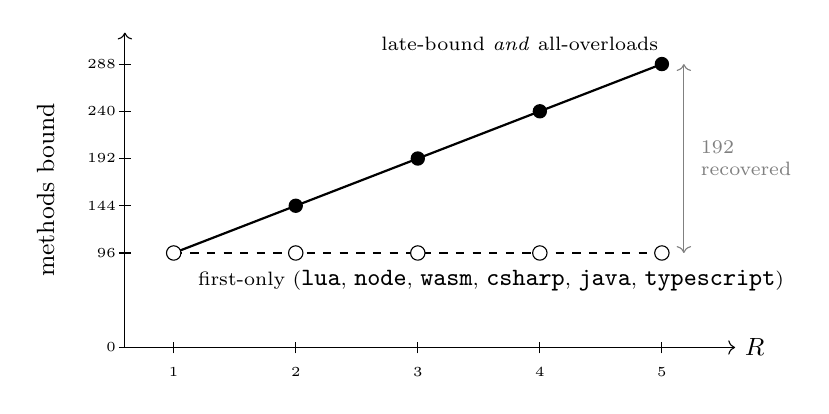
\begin{tikzpicture}[x=1.55cm, y=0.0125cm]
  % axes
  \draw[->] (0.6,0) -- (5.6,0) node[right,font=\small] {$R$};
  \draw[->] (0.6,0) -- (0.6,320);
  \foreach \y in {0,96,144,192,240,288}
    \draw (0.55,\y) -- (0.65,\y) node[left,font=\tiny,xshift=-2pt] {\y};
  \foreach \x in {1,2,3,4,5}
    \draw (\x,-6) -- (\x,6) node[below,font=\tiny,yshift=-6pt] {\x};
  \node[rotate=90,font=\small] at (-0.05,160) {methods bound};

  % late-bound / all-overloads (identical: they coincide)
  \draw[thick] (1,96) -- (2,144) -- (3,192) -- (4,240) -- (5,288);
  \foreach \p in {(1,96),(2,144),(3,192),(4,240),(5,288)}
    \fill \p circle (2.6pt);
  \node[font=\scriptsize,anchor=south east] at (5.05,292) {late-bound \emph{and} all-overloads};

  % first-only
  \draw[thick,dashed] (1,96) -- (5,96);
  \foreach \p in {(1,96),(2,96),(3,96),(4,96),(5,96)}
    \fill[white] \p circle (2.6pt);
  \foreach \p in {(1,96),(2,96),(3,96),(4,96),(5,96)}
    \draw \p circle (2.6pt);
  \node[font=\scriptsize,anchor=north] at (3.6,88) {first-only (\code{lua}, \code{node}, \code{wasm}, \code{csharp}, \code{java}, \code{typescript})};

  % the gap
  \draw[<->,gray] (5.18,96) -- (5.18,288);
  \node[font=\scriptsize,gray,anchor=west,align=left] at (5.24,192) {192\\recovered};
\end{tikzpicture}
\caption{E1: methods bound as the number of overloads per name grows
($C=8$, $N=6$). The first-only targets are flat --- their binding surface is a
name-keyed map, so a name can be registered once regardless of how many
overloads exist. The late-bound projection coincides with the library. The
overloads were never lost from the IR; they were lost by a projection that had
to commit at generation time.}
\label{fig:e1}
\end{figure}

\begin{table}[h]
\centering\small
\begin{tabular}{lrrrrr}
\toprule
overloads per name $R$ & 1 & 2 & 3 & 4 & 5 \\
\midrule
methods in the library                          & 96 & 144 & 192 & 240 & 288 \\
\code{python} / \code{nanobind} / \code{julia}  & 96 & 144 & 192 & 240 & 288 \\
\code{lua} / \code{node} / \code{wasm} / \code{csharp} / \code{java} & 96 & 96 & 96 & 96 & 96 \\
\code{typescript} (declares \code{node}'s module) & 96 & 96 & 96 & 96 & 96 \\
\code{dynamic} (late-bound)                     & 96 & 144 & 192 & 240 & 288 \\
\midrule
\textbf{recovered by late binding}              & 0 & \textbf{48} & \textbf{96} & \textbf{144} & \textbf{192} \\
\bottomrule
\end{tabular}
\caption{E1, methods bound. Two controls were clean in every configuration:
zero members were dropped for any reason other than the overload policy, and
zero were dropped by the reflective walk before a backend saw them --- so every
difference above is attributable to a backend decision, not to information loss
upstream.}
\label{tab:e1}
\end{table}

\paragraph{An instrument the experiment found broken.} On its first run E1
reported \code{typescript} as binding zero members in every configuration. The
backend recorded its skips but never called \code{note\_bound}, so its coverage
figure was structurally zero whatever it emitted --- a defect in the
instrumentation, not in the binding. The analysis detects this shape
(skips $>0$ with bound $=0$) and refuses to average it in, which is how it was
caught rather than published. It is now fixed, and the row above is the result:
\code{typescript} tracks \code{node} exactly, at 96 bound and $192$ overload
drops at $R=5$.

That it tracks \code{node} is the point rather than a coincidence. TypeScript
\emph{does} support declaration overloads, so nothing about the language forces
the policy; the \code{.d.ts} describes the N-API module, and declaring an
overload the module does not bind would promise the caller a method that is not
there. Its first-only policy is inherited from what it describes, which is why
it is listed apart from the five whose own binding surface is name-keyed.

\paragraph{Threats to validity.} The library is synthetic, and overload
multiplicity is controlled precisely because it is the independent variable ---
E5 measures a real API, where the distribution of overload-set sizes is whatever
it happens to be. The result also says nothing about cost: every recovered call
pays a name lookup and an overload-scoring pass, which E4 measures. The honest
summary is that late binding buys expressiveness with per-call time.

\subsection{E2 --- The cost of API evolution}
\label{sec:e2}

\paragraph{Design.} One synthetic library in three cumulative versions --- 10,
30 and 130 classes, each with four methods and three fields. Versions are strict
supersets, so ``what changed'' is a genuine diff rather than a reshuffle. Three
arms are generated for every version: the \emph{static} binding (pybind11,
N-API and sol2 together), the \emph{metadata tables} that are stage 1 of the
scriptable projection, and the \emph{scriptable binding} of
\code{rosetta::script} that is stage 2.

The static arm doubles as the stand-in for hand-written bindings: the emitted
pybind11 module is, line for line, what a developer would otherwise write. We
measure the size of that artifact, not the time to produce it --- this is an
upper bound on what automation removes, not a developer-hours study.

\paragraph{Result.} Table~\ref{tab:e2} reports it. Every relationship is exactly
linear over the measured range.

\begin{table}[h]
\centering\small
\begin{tabular}{lrrrl}
\toprule
 & 10 classes & 30 & 130 & fit \\
\midrule
\multicolumn{5}{l}{\itshape generated binding source (LOC)} \\
static binding                     & 763 & 2\,103 & 8\,803 & $93 + 67N$ \\
scriptable stage 1 --- tables      & 1\,106 & 3\,006 & 12\,506 & $156 + 95N$ \\
scriptable stage 2 --- the binding & 1\,208 & 1\,208 & 1\,208 & \textbf{constant} \\
\midrule
\multicolumn{5}{l}{\itshape human-authored manifest (lines)} \\
static                             & 53 & 133 & 533 & $13 + 4N$ \\
scriptable stage 2                 & 25 & 25 & 25 & \textbf{constant} \\
\midrule
\multicolumn{5}{l}{\itshape source files changed by the version bump} \\
static binding                     & --- & 4 & 4 & \\
scriptable stage 1 --- tables      & --- & 2 & 2 & \\
scriptable stage 2 --- the binding & --- & \textbf{0} & \textbf{0} & \\
\midrule
\multicolumn{5}{l}{\itshape generation wall-clock, driver compile (s)} \\
static                             & 3 & 5 & 14 & \\
scriptable stage 2                 & 5 & 5 & \textbf{5} & \\
\bottomrule
\end{tabular}
\caption{E2. The scriptable binding is byte-identical at 10 classes and at 130,
and its manifest never names a library class. Growing the library by 120 classes
changes zero of its source files.}
\label{tab:e2}
\end{table}

\paragraph{The result is not that it generates less code.} It generates
\emph{more}. Summed across both stages the scriptable arm produces 2\,314 LOC at
10 classes and 13\,714 at 130, against 763 and 8\,803 for the static binding:
the metadata tables cost more per class (95 LOC) than the pybind11 registration
they replace (67 LOC), and stage 2 adds a fixed 1\,208 LOC. Read purely as an
artifact-size question, the scriptable projection does not break even until
about seventeen classes, and never catches up in total bytes.

What changes is \emph{what has to change, and who writes it}. Three quantities
are constant in the size of the library: the binding's source, its manifest, and
its generation time. And the fixed 1\,208 LOC is not a per-library cost at all
--- it is a binding of \code{rosetta::script}, identical for every library that
has been through the \code{dynamic} backend, so it is paid once rather than once
per project. The static arm's $67N$ is paid again by every library.

\paragraph{What still scales.} The metadata tables regenerate on every version
bump and two of their files change each time. The scriptable projection makes
the \emph{binding} independent of the library; it does not make the pipeline
independent of it, and a claim of $O(1)$ maintenance for the whole chain would
be false. Section~\ref{sec:limitations} records this.

\paragraph{Threats to validity.} The library is uniform, so LOC per class is a
cleaner constant than a real API would give; what is tested is the scaling
relationship, not the constants. Only generation is measured --- compiling
12\,506 lines of tables is not free, and that cost is measured in
Section~\ref{sec:e3}.

\subsection{E3 --- Generation cost and scalability}
\label{sec:e3}

E1 and E2 measure what the pipeline \emph{produces}. E3 measures what running it
\emph{costs}, and where that cost sits.

\paragraph{Design.} A synthetic library with four independent size knobs ---
$C$ classes, $M$ method names per class, $F$ fields per class, $R$ overloads per
name --- giving $C\cdot(F + M\cdot R)$ reflected members. As in E1 every type is
marshalable by every backend and every class is copyable, so nothing is skipped
and emitted volume is a function of the knobs alone. Five sweeps vary one knob
each from a base point of $C=16$, $M=4$, $F=3$, $R=1$ and three targets: classes
$1\dots128$, methods $1\dots16$, fields $1\dots16$, overloads $1\dots5$, and ---
holding the library fixed --- targets $1, 3, 5, 10, 19$.

Four stages are timed separately: \code{rosetta\_gen} (manifest to driver
project), the CMake configure, the \emph{driver compile} with
\code{clang-p2996}, and the generator run. Only the driver compile is
reflective; the hypothesis is that it dominates. All figures are from one
machine (Apple M2 Pro, macOS 15.7, \code{clang-p2996} at \code{9ffb96e}) and the
noise floor, measured from configurations that should be identical, is
1.9--4.4\%.

\paragraph{Result: the reflective compile is the pipeline.} It is a median
\textbf{94\%} of wall-clock across all 28 configurations. The other stages do
not compete: \code{rosetta\_gen} takes 7\,ms, and the generator run --- which
writes the entire binding tree --- takes about 0.2\,s and shows \emph{no}
dependence on library size, because at these volumes it is process start-up and
file I/O. Emitting 15\,000 lines of bindings is not the expensive part of
generating them.

\paragraph{Result: linear, in every knob independently.} Figure~\ref{fig:e3}
pools every configuration that changes the library. The fit is $2.18\,\text{s} +
13.7\,\text{ms}$ per reflected member ($R^2 = 0.987$), and each sweep on its own
is linear to $R^2 \ge 0.997$. Because sweeps B, C and D each add exactly one
\emph{kind} of member, the pooled slope decomposes:

\begin{center}\small
\begin{tabular}{lrr}
\toprule
member added & ms per member & $R^2$ \\
\midrule
a field                        & 8.8  & 0.9991 \\
a method with a distinct name  & 14.1 & 0.9975 \\
an overload of an existing name & 16.0 & 0.9994 \\
\bottomrule
\end{tabular}
\end{center}

A method costs about $1.6\times$ a field, and an overload sibling costs slightly
more than a fresh name --- the walk has to spell out a signature to disambiguate
it, which is the same fact that made the \code{static\_cast} lines of
Listing~\ref{lst:five} awkward to transcribe by hand
(Section~\ref{sec:motivation}). Peak compiler memory grows
from 252\,MB at 7 members to 425\,MB at 896: enough to notice, not enough to
constrain.

The 2.18\,s intercept is the more practically relevant half of the fit. It is
the fixed cost of \code{<experimental/meta>}, the \rosetta{} headers, and all
nineteen backends --- which are linked into every driver whatever the manifest
asks for, because target selection is a runtime registry lookup. Below roughly
160 members, generation is dominated by a constant.

\begin{figure}[h]
\centering
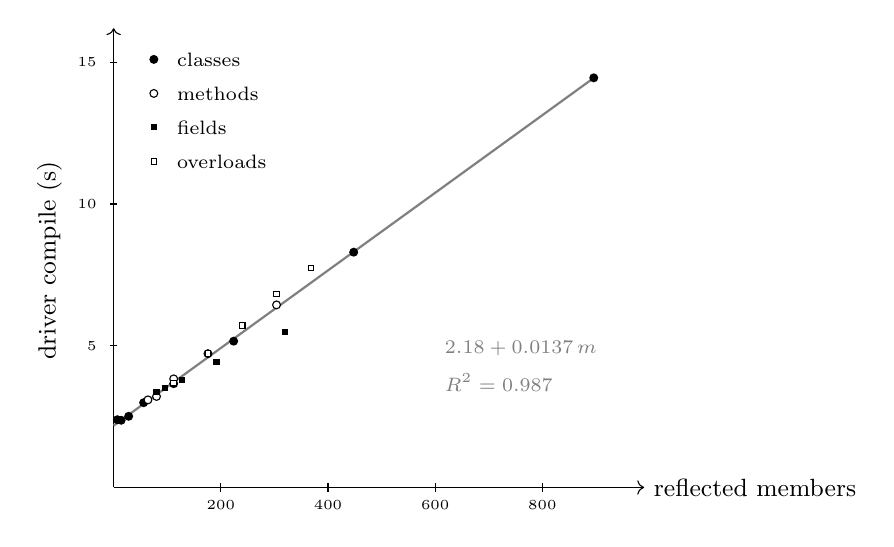
\begin{tikzpicture}[x=0.0068cm, y=0.36cm,
  mA/.style={circle, fill=black, inner sep=1.15pt},
  mB/.style={circle, draw, fill=white, inner sep=1.0pt},
  mC/.style={rectangle, fill=black, inner sep=1.1pt},
  mD/.style={rectangle, draw, fill=white, inner sep=1.0pt}]
  \draw[->] (0,0) -- (990,0) node[right,font=\small] {reflected members};
  \draw[->] (0,0) -- (0,16.2);
  \foreach \x in {200,400,600,800}
    \draw (\x,-0.16) -- (\x,0.16) node[below,font=\tiny,yshift=-3pt] {\x};
  \foreach \y in {5,10,15}
    \draw (-7,\y) -- (7,\y) node[left,font=\tiny,xshift=-4pt] {\y};
  \node[rotate=90,font=\small] at (-120,8) {driver compile (s)};

  % pooled least-squares fit: 2.18 + 0.01369 m
  \draw[gray,thick] (0,2.18) -- (900,14.50);
  \node[font=\scriptsize,gray,anchor=west] at (600,4.9)
       {$2.18 + 0.0137\,m$};
  \node[font=\scriptsize,gray,anchor=west] at (600,3.7) {$R^2=0.987$};

  \foreach \p in {(7,2.39),(14,2.37),(28,2.51),(56,2.99),(112,3.66),
                  (224,5.16),(448,8.30),(896,14.45)} \node[mA] at \p {};
  \foreach \p in {(64,3.09),(80,3.21),(112,3.83),(176,4.72),(304,6.44)}
    \node[mB] at \p {};
  \foreach \p in {(80,3.36),(96,3.52),(128,3.80),(192,4.41),(320,5.47)}
    \node[mC] at \p {};
  \foreach \p in {(112,3.68),(176,4.72),(240,5.71),(304,6.82),(368,7.74)}
    \node[mD] at \p {};

  % legend, in the empty region above the line
  \node[mA] at (75,15.1) {}; \node[font=\scriptsize,anchor=west] at (100,15.1) {classes};
  \node[mB] at (75,13.9) {}; \node[font=\scriptsize,anchor=west] at (100,13.9) {methods};
  \node[mC] at (75,12.7) {}; \node[font=\scriptsize,anchor=west] at (100,12.7) {fields};
  \node[mD] at (75,11.5) {}; \node[font=\scriptsize,anchor=west] at (100,11.5) {overloads};
\end{tikzpicture}
\caption{E3: driver compile time against reflected members, pooling the four
sweeps that change the library. Whichever knob moved the member count, the cost
lands on the same line --- the walk is per-member, and no knob is
disproportionately expensive. The fields sweep sits slightly below it and the
overloads sweep slightly above, which is the per-kind difference reported above.}
\label{fig:e3}
\end{figure}

\paragraph{Result: the walk is per-library, not per-target.} This is the claim
Section~\ref{sec:ir} makes architecturally, and it is the one E3 can falsify.
Holding the library fixed and asking for 1, 3, 5, 10 and then all 19 targets,
the driver compile is 3.60--3.67\,s --- a 1.9\% spread, below the noise floor
--- while the emitted output goes from 1\,582 lines in 6 files to 9\,998 lines
in 85, and the generator run stays at roughly 0.2\,s. \emph{The eighteenth
additional target is free at generation time.} One \code{consteval} walk builds
the IR; the backends are ordinary functions that consume it at run time, so the
per-target cost is text emission measured in milliseconds. Table~\ref{tab:e3}
gives the numbers.

\begin{table}[h]
\centering\small
\begin{tabular}{rrrrr}
\toprule
targets & driver compile (s) & generator run (s) & emitted lines & files \\
\midrule
1  & 3.65 & 0.16 & 1\,582 & 6 \\
3  & 3.67 & 0.20 & 2\,027 & 15 \\
5  & 3.60 & 0.30 & 2\,460 & 21 \\
10 & 3.62 & 0.17 & 5\,553 & 58 \\
19 & 3.64 & 0.17 & 9\,998 & 85 \\
\bottomrule
\end{tabular}
\caption{E3, sweep E. Identical library throughout; only the number of requested
targets changes. A $6.3\times$ increase in emitted output costs nothing
measurable in reflection time.}
\label{tab:e3}
\end{table}

\paragraph{Result: the metadata tables cost 287 bytes per member.} The one thing
E3 compiles beyond the driver is \code{auto\_dynamic.cpp}, at \code{-O2} with the
\emph{system} compiler --- the tables are stock C++20, which is the point of the
dynamic backend. Their footprint is $5\,228\,\text{B} + 287\,\text{B}$ per member
($R^2 = 0.991$), split roughly evenly between the descriptor tables with their
strings and the emitted per-member call thunks. The largest library measured,
896 members, produces 272\,kB. That is the price of the runtime meta-object
model in the binary, and Section~\ref{sec:e4} prices it per call.

That compile is also the cost E2 deferred to here. It runs at
$0.51\,\text{s} + 1.32\,\text{ms}$ per member --- an order of magnitude cheaper
per member than the reflective walk that produced the tables, which is what
one would hope from code whose entire design is that it is data rather than
reflection.

\paragraph{What this bounds.} A 1\,000-member library --- larger than most
single-header scientific APIs --- regenerates in about 16\,s for as many targets
as one cares to name, on one core, and adds a quarter of a megabyte if the
dynamic projection is wanted. That is a build step, not a research problem. The
honest caveat is that it is \emph{serial}: the driver is one translation unit by
construction, so the reflective compile cannot use the other eleven cores of the
machine it was measured on.

\paragraph{Threats to validity.} The library is uniform, so cost per member is a
cleaner constant than a real API would give; the scaling relationship is what is
tested, not the constants. One machine and one revision of a research compiler
that is not tuned for compile speed: the shape of the curve travels, the seconds
do not. And E3 stops after generation, with the single metadata compile as the
deliberate exception --- \emph{compiling} the emitted bindings costs
considerably more than generating them, but that is a cost of pybind11, N-API
and embind rather than of \rosetta.

\subsection{E4 --- Runtime overhead}
\label{sec:e4}

E1 showed that late binding recovers API surface. E4 prices it.

\paragraph{Design: two layers.} Measuring only from a host language would
confound two independent costs. Layer~A runs entirely in C++ --- \emph{direct}
call, \emph{dyn} (resolved by name on every call), and \emph{dyn-cached} (the
\code{MetaMethod} resolved once and reused) --- and so isolates late binding
with no interpreter present. Layer~B runs the same operations from Python
through the generated pybind11 module and through the scriptable meta-object
binding, and so measures late binding \emph{and} the language boundary together.
The difference between the layers is the interpreter's share.

The cached arm is not a strawman-avoidance device: \code{dynamic.h} explicitly
recommends it (``the returned pointer is stable for the process, so a wrapper
should cache it per call site''), so reporting only the uncached path would
price a usage the documentation tells the reader not to write.

\begin{table}[h]
\centering\small
\begin{tabular}{lrrrrr}
\toprule
 & \multicolumn{3}{c}{layer A --- C++} & \multicolumn{2}{c}{ratio} \\
\cmidrule(lr){2-4}\cmidrule(lr){5-6}
operation & direct & dyn & dyn-cached & dyn & cached \\
\midrule
trivial-call   & 3.6\,ns & 51.5\,ns & 4.2\,ns & 14.4$\times$ & \textbf{1.2$\times$} \\
field-get      & 3.6\,ns & 10.8\,ns & 4.2\,ns & 3.0$\times$ & \textbf{1.2$\times$} \\
field-set      & 3.6\,ns & 75.2\,ns & 4.2\,ns & 21.0$\times$ & \textbf{1.2$\times$} \\
3-arg-call     & 3.6\,ns & 159.2\,ns & 14.6\,ns & 44.4$\times$ & 4.1$\times$ \\
object-return  & 3.4\,ns & 187.7\,ns & 107.4\,ns & 54.8$\times$ & 31.3$\times$ \\
vector-1000    & 386.6\,ns & 17.5\,\textmu s & 7.8\,\textmu s & 45.4$\times$ & 20.2$\times$ \\
overload-3way  & 3.6\,ns & 629.0\,ns & 14.2\,ns & \textbf{175.3$\times$} & 4.0$\times$ \\
\midrule
 & \multicolumn{3}{c}{layer B --- from Python} & & \\
\cmidrule(lr){2-4}
operation & pybind11 & scriptable & & \multicolumn{2}{c}{ratio} \\
\midrule
trivial-call   & 86.9\,ns & 467.0\,ns & & \multicolumn{2}{c}{5.4$\times$} \\
field-get      & 87.6\,ns & 317.3\,ns & & \multicolumn{2}{c}{3.6$\times$} \\
field-set      & 92.6\,ns & 436.9\,ns & & \multicolumn{2}{c}{4.7$\times$} \\
3-arg-call     & 119.8\,ns & 895.6\,ns & & \multicolumn{2}{c}{7.5$\times$} \\
object-return  & 245.0\,ns & 615.2\,ns & & \multicolumn{2}{c}{2.5$\times$} \\
vector-1000    & 17.1\,\textmu s & 42.9\,\textmu s & & \multicolumn{2}{c}{2.5$\times$} \\
overload-3way  & 108.4\,ns & 1\,216\,ns & & \multicolumn{2}{c}{11.2$\times$} \\
\bottomrule
\end{tabular}
\caption{E4. Layer A isolates late binding; layer B adds the language boundary.
Best of five; repeatability across consecutive runs $\pm 1.5\%$.}
\label{tab:e4}
\end{table}

\paragraph{Most of the cost is name lookup, and caching removes it.} For the
three cheapest operations, caching the resolved member brings late binding to
$1.2\times$ a direct C++ call. The thunk is not the problem; finding it is.

\paragraph{Overload resolution is the expensive lookup --- and it is the one
E1 credits.} Scoring a three-candidate set costs 629\,ns uncached against
14\,ns cached, and is the worst ratio in the experiment at $175\times$ direct.
Read with Section~\ref{sec:e1}, this is the whole trade in two numbers: late
binding recovers two thirds of the API on name-keyed targets, and scoring the
candidates at every call is what that recovery costs. Caching the resolution
keeps the expressiveness at $4.0\times$.

\paragraph{Marshalling cannot be cached away.} Object return remains at
$31\times$ and the 1000-element vector at $20\times$ even fully cached and
pre-boxed, because the cost is boxing each value into an \code{Any} rather than
finding the method. This is the floor of the dynamic model, and no amount of
call-site caching moves it.

\paragraph{From a host language the penalty shrinks.} Crossing the boundary
already costs 87--245\,ns, so a $175\times$ C++ ratio becomes $11.2\times$ seen
from Python and the bulk-data case falls to $2.5\times$. The interpreter, not
the meta-object model, is the dominant cost of scripting a C++ library.

\paragraph{The rule, in numbers.} At 317--467\,ns per scriptable operation, a
property panel with 100 fields costs roughly 32\,\textmu s --- imperceptible ---
while a one-million-element loop costs 0.47\,s. \code{docs/PIPELINE.md} claims
in prose that the model is right for menus, panels and glue and wrong for bulk
data; the measured boundary is four to five orders of magnitude of call count,
not a subtle judgement.

\paragraph{Threats to validity.} One machine, one compiler: the ratios travel
further than the absolute figures. Microbenchmarks measure microbenchmarks --- a
real property panel interleaves these calls with layout and I/O that dwarf both
arms. The scriptable arm returns an outcome object where the static arm returns
a bare float; that allocation is part of the API and is deliberately included
rather than subtracted.

\subsection{E5 --- Coverage on a real library}
\label{sec:e5}

E1--E4 measure synthetic libraries, which are built to isolate one variable and
therefore cannot answer what a real API contains. E5 points the pipeline at one
that was never written with binding in mind.

\paragraph{Subject.} PMP, the Polygon Mesh Processing
library~\cite{pmp}, unmodified. It is not a library either author wrote --- the
relevant objection to using \code{geogram} here --- and it is small enough to
bind \emph{exhaustively}, which is the property that matters: at this size the
experiment can bind everything and publish the breakdown, rather than choosing a
subset and inviting the reader to trust the choice.

\paragraph{Design: the denominator is the difficulty.} ``What fraction of an API
binds'' is a measurement only if somebody other than the experimenter decides
what the API \emph{is}. The frame is therefore read from clang's own AST: every
class, class template, enum and free function declared in namespace \code{pmp}
by a header under \code{src/pmp/}, excluding the OpenGL viewers. Templates stay
\emph{in} the frame --- a template cannot be named in a manifest, so filtering
them out would raise every percentage below without changing a fact.

Two arms differ in one variable, who chose the entries:
\emph{exhaustive}, generated mechanically from that frame, and \emph{curated},
a real hand-written manifest for the same library, retargeted so both emit the
same ten backends. The exhaustive arm makes exactly two mechanical concessions,
both to the manifest format rather than to taste: an overloaded name carries a
signature (\code{\^{}\^{}pmp::centroid} is ill-formed once the name is declared
twice), and classes are topologically sorted so a base precedes its derived
classes.

\paragraph{Result: it works, unattended.} Nineteen classes, two enums and 91
free functions from an unmodified third-party library reach a driver that
compiles and runs with no hand-tuning at all. The build is not error-tolerant by
construction: compiling the emitted generator is exactly where a class the walk
mishandles would surface as a build failure, which is the outcome
Section~\ref{sec:coverage} claims cannot happen, so the harness treats a
non-zero exit there as the finding rather than swallowing it. It did not occur.

\paragraph{Result: a quarter of the surface is templates, and they are not
spread out.} Of 166 declared entities, 120 are nameable and 46 are templates ---
28\% out of reach before any backend is consulted. But 39 of those 46 are in a
single header, \code{mat\_vec.h}, the library's vector and matrix value types;
the algorithm headers contribute exactly one. The useful form of the finding is
therefore not ``templates block a quarter of the API'' but that
\emph{the templates sit in the value types and the property system, while the
algorithm surface a script user actually calls is essentially template-free}.
That is a claim about where a reflection-based binder loses, and it is more
actionable than the aggregate.

\paragraph{Result: real overload multiplicity is far below E1's sweep.}
Section~\ref{sec:e1} sweeps overloads-per-name because a synthetic library has
no opinion about it. Here the value is measured: PMP's 91 free-function names
carry 99 declarations, so a first-only policy costs \textbf{8 of 99 (8\%)} of the
free-function surface, against the two thirds E1 reports at its worst swept
case. The mechanism E1 isolates is real and the recovery is real; at
free-function scope \emph{this} library barely exercises it. Class members are
where the multiplicity actually lives --- every first-only target drops 27
members to \code{overload\_not\_expressible} --- which is the honest shape of
E1's result on a real API: significant, and an order of magnitude below the
headline the sweep's endpoint suggests.

\begin{table}[h]
\centering\small
\begin{tabular}{lrrrr}
\toprule
target & members & functions & fns skipped & bound/req. \\
\midrule
\code{python} / \code{nanobind} / \code{julia} & 123 & 64 & 27 & 75\% \\
\code{node}       & 106 & 82 & 9  & 76\% \\
\code{lua} / \code{wasm} & 104 & 64 & 27 & 68\% \\
\code{csharp} / \code{java} & 61 & 2 & 89 & 25\% \\
\code{dynamic} (late-bound) & 141 & 54 & 37 & 73\% \\
\bottomrule
\end{tabular}
\caption{E5, exhaustive arm. \code{typescript} is omitted: it records bound
fields where the language backends record methods only, so its member column is
over a different denominator. The C\#/Java collapse is one cause --- their
boundary is JSON, and 89 of 91 free functions name a type with no JSON
marshalling.}
\label{tab:e5}
\end{table}

\paragraph{Result: curation subtracts reach rather than adding it.} The
exhaustive arm binds strictly more than the curated one on every target, by 23
to 78 entities. This is worth stating carefully, because the intuitive
expectation is the reverse --- that a hand-written manifest exists to rescue
what automation cannot manage. It does not: it exists to choose. The curated
manifest omits property containers, handles and iterators that bind perfectly
well and that no script user would call, and in exchange its \code{out\_params}
and \code{sequences} give nicer signatures to the members it does keep. E5
measures reach; the two arms point in opposite directions on reach and quality,
and only the first is a number.

\paragraph{A limit that sits above the backends.} Eight free-function
declarations never reached any backend: two manifest entries binding under one
exposed name are a \code{rosetta\_gen} error, so only one overload of a
free-function name can be requested at all. This is stricter than the per-target
policy of Section~\ref{sec:overloads} and it applies to \emph{every} target,
including pybind11 and jlcxx, which would have taken the whole set. It is a
limitation of the manifest format, not of any target language, and E5 is what
surfaced it.

\paragraph{Two instruments this experiment repaired.} E5 was not measurable as
designed until both were fixed, and both say something about
\code{coverage.json} rather than about PMP. First, \emph{no backend recorded
free functions at all} --- the report covered class members only, which on a
library whose algorithms are free functions over one data structure meant 99 of
120 nameable entities were invisible to it. Second, the \code{typescript}
backend emitted free-function declarations through no visibility gate,
promising callers functions the N-API module does not bind. Both are fixed;
the free-function counts above are cross-validated against emitted output (the
pybind11 module contains exactly the 64 \code{m.def} calls the report claims).
Section~\ref{sec:coverage} asserts that every unexposed member is recorded with
a reason. Before E5 that was true of methods and false of free functions.

\paragraph{Threats to validity.} One library, and a well-behaved one: PMP is
modern, clean C++17, and a template-heavy or macro-heavy API would give
different constants and possibly a different shape. The frame excludes
\code{viewers/}, which needs an OpenGL context --- the one judgement in it, and
recorded in the output. Coverage counts entities rather than usefulness, which
is what makes the curation comparison a statement about reach only. And the
member column is not comparable across all targets, for the field-recording
asymmetry noted under Table~\ref{tab:e5}.

% =====================================================================
\section{Case study: one library, six consumers, one new class}
\label{sec:case}

Sections~\ref{sec:eval}'s experiments each isolate one variable. This section
does the opposite: it takes the whole pipeline as a user meets it, and asks what
happens when the library moves.

\subsection{The library and its consumers}

\code{scene.h} is 233 lines of ordinary C++ --- no \rosetta{} header, no
attribute, no base class. Every \code{doc}, \code{range}, \code{combobox} and
\code{readonly} hint lives out of line in JSON side-cars named by the manifest,
so the header is what an unmodified third-party library looks like. It declares
a value type (\code{Vec3}), a document (\code{Mesh}, carrying real geometry
behind \code{positions()}/\code{triangles()}), and an enum.

One \code{dynamic} projection of it feeds six consumers, none of which is
compiled against \code{scene.h} and none of which names a bound type:

\begin{itemize}\setlength{\itemsep}{1pt}
  \item a terminal interpreter and a registry inspector, both in C++;
  \item a Qt viewer --- 3D view, generated property panel, completing console;
  \item Python, Lua and Node drivers, and a \code{three.js} browser editor over
        WebAssembly, all going through the \emph{scriptable} projection: a
        binding of \code{rosetta::script} itself, which names no library class
        at all (Section~\ref{sec:dynamic}).
\end{itemize}

\paragraph{Why that second group matters.} The C++ consumers each contain a
hand-written walker over the metadata --- \code{interp.h}, the property panel,
the Add menu, and elsewhere in the tree an ImGui and a QML one: five walkers,
one per toolkit, all traversing the same tables. Binding the reflection API
instead moves that walk into the language whose interface it builds, so the Qt
panel's dispatch is written in Python where the Qt binding already lives. We
resist the tempting line count here: the Python spec-builder is 27 lines against
the C++ panel's 401, but the C++ file also constructs and wires the widgets,
which the Python one hands to PyQt. The defensible statement is structural, not
a ratio --- \emph{one walker per toolkit becomes one walker per toolkit in that
toolkit's own language}, and the walker stops being C++.

\subsection{Growing the library}

The library then gains a third kind of thing: a \emph{solver}.
\code{scene::Relaxer} improves the shape of a triangle mesh by tangential
Laplacian relaxation --- each pass moves every vertex a fraction \code{step}
toward the centroid of its one-ring, which equalises edge lengths and so drives
triangles toward equilateral. The displacement is projected onto the vertex
tangent plane, which is what stops the classic collapse of naive Laplacian
smoothing: on the Stanford bunny at 40 passes, the bounding-box diagonal loses
$1.05\%$ with that projection off and $0.01\%$ with it on, for the same quality
gain.

A solver is the interesting case for this projection because it is mostly
\emph{tuning}: four public parameters with declared ranges, three read-only
outputs, and one method that runs for a while and mutates something else. That
is exactly a property sheet, and nobody writes one.

\begin{table}[h]
\centering\small
\begin{tabular}{lrrr}
\toprule
 & mean quality & worst triangle & bbox diagonal \\
\midrule
bunny, before      & 0.834 & 0.014 & 1.6072 \\
bunny, after 25 passes & \textbf{0.912} & \textbf{0.102} & 1.6076 \\
\bottomrule
\end{tabular}
\caption{The solver, driven through the dynamic model. Quality is
$4\sqrt{3}A/(a^2{+}b^2{+}c^2)$, which is 1 for an equilateral triangle. The
worst triangle improves by $7\times$ while the silhouette does not move.
Identical figures are produced from the C++ console and from Python, because
both call the same tables.}
\label{tab:e6}
\end{table}

\paragraph{What it cost downstream: nothing.} Adding the solver touched three
files, all of them the library's own --- \code{scene.h}, one annotation
side-car, and one line of the manifest naming the new class. No consumer
changed: not the Qt viewer, not the property panel, not the console, not the
terminal interpreter, and none of the five scriptable drivers. Yet the generated
inspector lists the solver's fields with their ranges and read-only flags, the
console runs it (Figure~\ref{fig:e6}), and the Python driver's property sheet
grows its rows.

\begin{figure}[h]
\centering
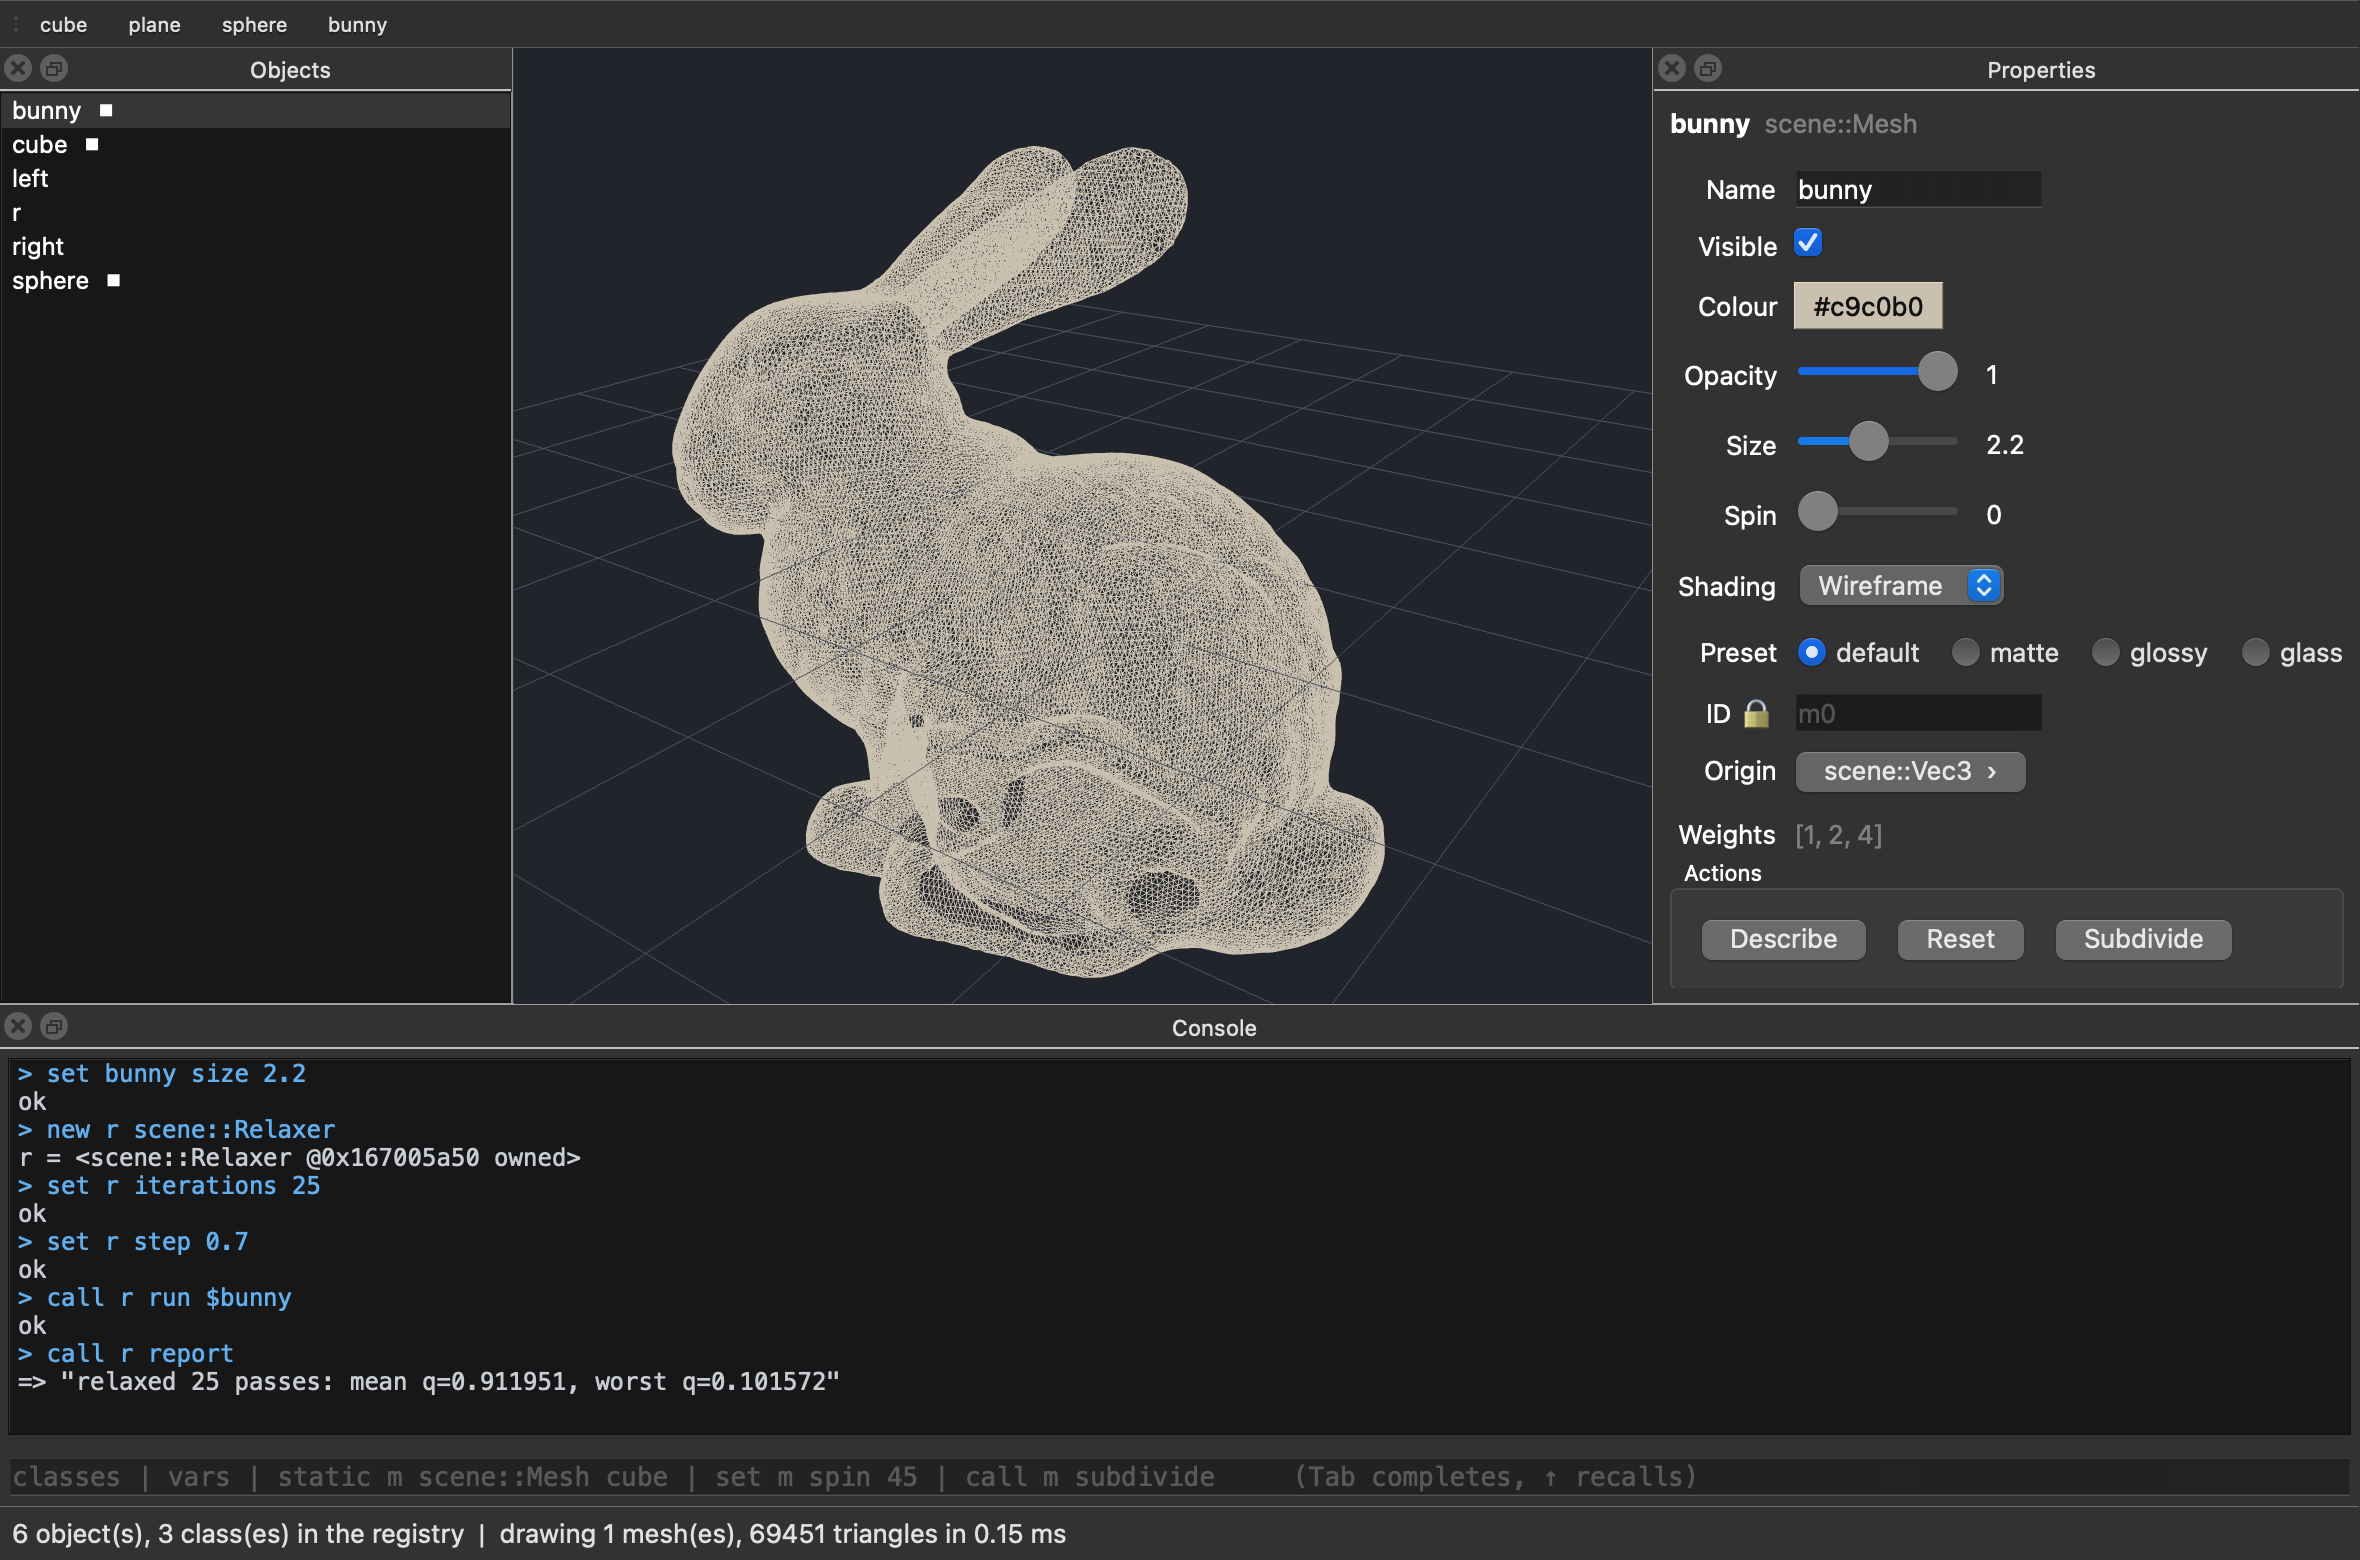
\includegraphics[width=\textwidth]{figures/e6-viewer.png}
\caption{The Qt viewer after the library grew a solver. The console session
creates a \code{scene::Relaxer}, sets its parameters and calls \code{run} on the
bunny; the object list gains \code{r}; the view redraws from the mutated mesh.
Nothing in \code{qt/} was recompiled against the solver, and nothing in it
mentions one --- the window is built by querying metadata that grew.}
\label{fig:e6}
\end{figure}

\subsection{The claim, checked rather than asserted}

A case study can assert anything, so this one is also a test
(\code{E6-case-study/}). The same library goes through the pipeline twice,
differing only in whether the manifest lists \code{Relaxer}, and the generated
artifacts are compared. The prediction is deliberately two-sided, because a
byte-identity test invites a vacuous pass:

\begin{itemize}\setlength{\itemsep}{1pt}
  \item the \emph{metadata} must differ --- 4 stage-1 files change, and
        \code{Relaxer} is present in the ``after'' tables and absent from
        ``before'';
  \item the \emph{binding} must not --- and 0 of 18 stage-2 files change,
        across 4\,173 generated lines.
\end{itemize}

Both hold. That second number is the point of Section~\ref{sec:dynamic} stated
as an artifact: the binding a host imports is a binding of the reflection API,
so the library grew and the thing every consumer depends on did not move a byte.
E2 measures the same property as a file-count across a $13\times$ growth; this
measures it as byte-identity across one concrete, human-sized change, and fails
the run if it ever stops being true.

\paragraph{What this does not show.} The harness compares generated artifacts;
that the hand-written consumers still work rests on the version-control evidence
above, which is weaker. The library is ours --- a demonstration library small
enough for a reader to hold in their head --- so the third-party evidence stays
in Section~\ref{sec:e5}. And the outline for this section once promised a Julia
arm; the \emph{scriptable} projection ships value casters for Python, Lua, Node
and WebAssembly but not Julia, so that arm does not exist and is not claimed.

% =====================================================================
\section{Limitations}
\label{sec:limitations}

\begin{enumerate}
  \item \textbf{Research toolchain.} Stage 1 requires \code{clang-p2996}. Stages
    0 and 2--3 do not, so the emitted artifacts outlive the fork --- but a
    project cannot re-generate without it.
  \item \textbf{Two targets are not reflection-free.} The claim in
    Section~\ref{sec:pipeline} holds for seventeen of the nineteen backends.
    The \code{rest} and \code{json} backends emit projects whose sources include
    a \emph{runtime visitor} that still splices reflections when the binding is
    compiled, and their generated \code{CMakeLists.txt} accordingly requests
    C++26. This is a design choice rather than an oversight --- reflecting at
    binding-compile time keeps those two emitters very small, because the
    per-member code is written once as a template instead of being expanded by
    the generator --- but it is a real trade of deployment simplicity for
    generation simplicity, and it means those two targets inherit the fork
    dependency. The distinction is worth naming: a backend may spend the IR
    either at generation time or at binding-compile time, and only the former
    yields a reflection-free artifact.
  \item \textbf{Inline annotations forfeit the reflection-free property.} An
    annotation written in a user header pulls \code{<experimental/meta>} into
    that header, so the calling pass needs C++26 as well. Out-of-line
    annotations exist precisely to avoid this and are load-bearing, not
    cosmetic.
  \item \textbf{Type casters are hand-written.} Reading a host-language value is
    irreducibly per-language: roughly nine methods per language, plus the
    reading half.
  \item \textbf{The scriptable projection is not $O(1)$ end to end.} Only the
    binding is independent of the library: the metadata tables still regenerate
    on every change, growing at 95 LOC per class, and the scriptable arm emits
    \emph{more} total code than the static one at every size we measured
    (Section~\ref{sec:e2}). What is constant is the binding, its manifest and
    its generation time --- not the pipeline.
  \item \textbf{Dynamic dispatch has a real cost.} Linear name lookup plus
    overload scoring per access. Inappropriate for inner loops; a resolved
    method handle is stable for the process and can be cached.
  \item \textbf{A vestigial type in each module.} Bindability is decided at
    generation time and cannot know that a type caster will exist later, so the
    boxed-value type must remain in the bound class list even though nothing
    ever produces it directly. One unused type per module.
  \item \textbf{Coverage measures exposure, not correctness.} A bound method can
    still be wrong; \code{coverage.json} counts what crossed the boundary, not
    whether it behaves.
  \item \textbf{No formal semantics.} The IR is defined by its implementation.
\end{enumerate}

% =====================================================================
\section{Related work}
\label{sec:related}

\gap{Draft the prose around Table~\ref{tab:related}; citations to be completed.}

\begin{table}[h]
\centering\footnotesize
\begin{tabular}{lccccc}
\toprule
system & type discovery & header intrusion & targets & runtime model & coverage \\
\midrule
SWIG~\cite{swig}            & own parser        & \code{.i} file & many & no & no \\
pybind11~\cite{pybind11}    & hand-written      & none & 1 & no & --- \\
nanobind~\cite{nanobind}    & hand-written      & none & 1 & no & --- \\
Qt moc~\cite{qt}            & own parser        & \code{Q\_OBJECT} & 1 & \textbf{yes} & no \\
Graphite/GOM~\cite{graphite}& manual registration & macros & Lua $+$ GUI & \textbf{yes} & no \\
Unreal UHT~\cite{unreal}    & own parser        & \code{UCLASS} & Blueprint & \textbf{yes} & no \\
cppyy~\cite{cppyy}          & Clang JIT         & none & 1 & yes & no \\
Clang-AST generators        & Clang AST         & none & 1--2 & no & partial \\
\midrule
\textbf{\rosetta}           & \textbf{language-native} & \textbf{none} & \textbf{19} & \textbf{yes} & \textbf{yes} \\
\bottomrule
\end{tabular}
\caption{Positioning. Two columns carry the delta --- language-native discovery
with no header intrusion, and both projections from one description. Every prior
system has at most one of them.}
\label{tab:related}
\end{table}

The nearest prior art is not another binding generator but the meta-object
systems: Qt's, Graphite's GOM, and Unreal's. Each demonstrated, long before
C++26, that a runtime object model can drive scripting and generated user
interfaces, and \rosetta's dynamic projection is explicitly a descendant of that
idea. What each of them requires is a \emph{separate description}: a macro
vocabulary in the header and a bespoke parser, or manual registration calls.
\rosetta's contribution against this line is that the description is the C++
source itself, read by the compiler, on headers that need no modification --- and
that the same description simultaneously produces the static bindings, which the
meta-object systems do not attempt.

Against the binding-generator line --- SWIG, pybind11, nanobind, Clang-AST
generators --- the delta is the opposite one. Those systems produce good
bindings for one or two targets, but each carries either a C++ front-end that
must track the language or a per-class hand-written specification, and none
produces a runtime object model. \rosetta{} does not claim better Python
bindings than pybind11 or nanobind; it claims that reaching the nineteenth target should not
cost nineteen times the first.

% =====================================================================
\section{Conclusion}
\label{sec:conclusion}

\gap{Write last.}

\todo{Restate: reflection as an interface description mechanism; one IR, two
projections; resolution time as the axis that explains their difference;
coverage as a measurable property of an interface. Close on the case study.}

% =====================================================================
\section*{Availability}
\rosetta{} is available at \url{https://github.com/rosetta-bindings/rosetta}
under the MIT licence. \todo{archive a release DOI (Zenodo) before submission}

% =====================================================================
\bibliographystyle{plain}
\bibliography{rosetta}

\end{document}
